\documentclass[tikz,border=5mm]{standalone}
\usepackage{tikz}
\usetikzlibrary{arrows.meta, positioning, shapes.geometric, calc, backgrounds, fit, matrix, patterns, decorations.pathmorphing, decorations.markings, shadows}

% --- COLOR DEFINITIONS ---
\definecolor{Garnet}{HTML}{73000A}
\definecolor{CSecondaryRed}{HTML}{CC2E40}
\definecolor{CBlue}{HTML}{466A9F}
\definecolor{CDark}{HTML}{1F414D}
\definecolor{COlive}{HTML}{65780B}
\definecolor{CLime}{HTML}{CED318}
\definecolor{CGold}{HTML}{A49137}
\definecolor{CGrayLight}{HTML}{E5E5E5}
\definecolor{CGrayDark}{HTML}{555555}
\definecolor{CWhite}{HTML}{FFFFFF}

\begin{document}

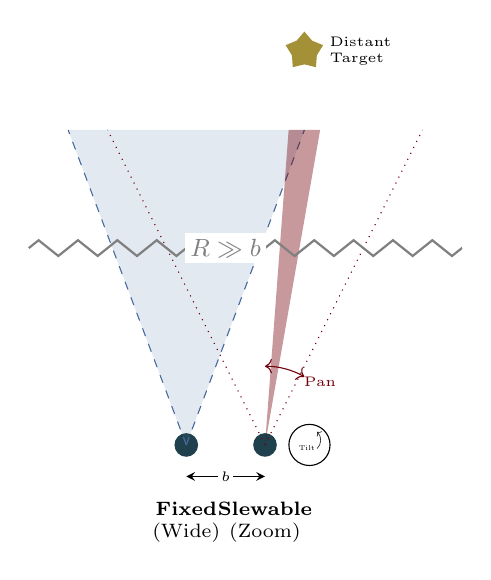
\begin{tikzpicture}
    % Cameras
    \coordinate (C1) at (-0.5, 0);
    \coordinate (C2) at (0.5, 0);
    
    % Camera Bodies
    \fill[CDark] (C1) circle (0.15);
    \fill[CDark] (C2) circle (0.15);
    
    % Baseline annotation
    \draw[<->, >=stealth, thin] (-0.5, -0.4) -- (0.5, -0.4) node[midway, fill=white, inner sep=1pt, font=\tiny] {$b$};
    
    % Fixed FoV (Camera 1)
    \fill[CBlue, opacity=0.15] (C1) -- (-2, 4) -- (1, 4) -- cycle;
    \draw[CBlue, dashed] (C1) -- (-2, 4);
    \draw[CBlue, dashed] (C1) -- (1, 4);
    
    % Slew Range (Camera 2) - The potential area
    \draw[Garnet, dotted, thin] (C2) -- (-1.5, 4);
    \draw[Garnet, dotted, thin] (C2) -- (2.5, 4);
    \draw[<->, Garnet, thin] (0.5, 1) arc (90:60:1);
    \node[Garnet, font=\tiny] at (1.2, 0.8) {Pan};
    
    % Zoom Beam (Camera 2) - Active narrow beam
    \fill[Garnet, opacity=0.4] (C2) -- (0.8, 4) -- (1.2, 4) -- cycle;
    
    % Distance Break
    \draw[decoration={zigzag, segment length=5mm, amplitude=1mm}, decorate, thick, gray] (-2.5, 2.5) -- (3, 2.5);
    \node[fill=white, inner sep=2pt, font=\small, text=gray] at (0, 2.5) {$R \gg b$};
    
    % Object
    \node[star, star points=5, fill=CGold, minimum size=0.5cm] (Obj) at (1.0, 5) {};
    \node[right, font=\tiny, align=left] at (Obj.east) {Distant\\Target};
    
    % Tilt Indicator Icon (Side View graphic next to Cam 2)
    \node[draw, circle, inner sep=1pt, scale=0.5, anchor=west] at (0.8, 0) {
        \tikz{
            \draw[->] (0,0) arc (-45:45:0.3);
            \node[font=\tiny, left] at (0,0) {Tilt};
        }
    };
    
    % Labels
    \node[below=0.6cm, align=center, font=\scriptsize] at (C1) {\textbf{Fixed}\\(Wide)};
    \node[below=0.6cm, align=center, font=\scriptsize] at (C2) {\textbf{Slewable}\\(Zoom)};
\end{tikzpicture}

\end{document}
